\documentclass[oneside,11pt]{book}
\usepackage[letterpaper]{geometry}
\usepackage{amsmath,amsthm,amssymb}
\usepackage{scalerel}
\usepackage{esint}
\usepackage{hyperref}

\hypersetup{
    colorlinks=true,
    urlcolor=cyan,
    pdftitle={Electromagnetism}
}

\renewcommand{\b}{\mathbf}
\newcommand{\h}[1]{\mathbf{\hat{#1}}}
\def\r{{\mbox{$\resizebox{.09in}{.08in}{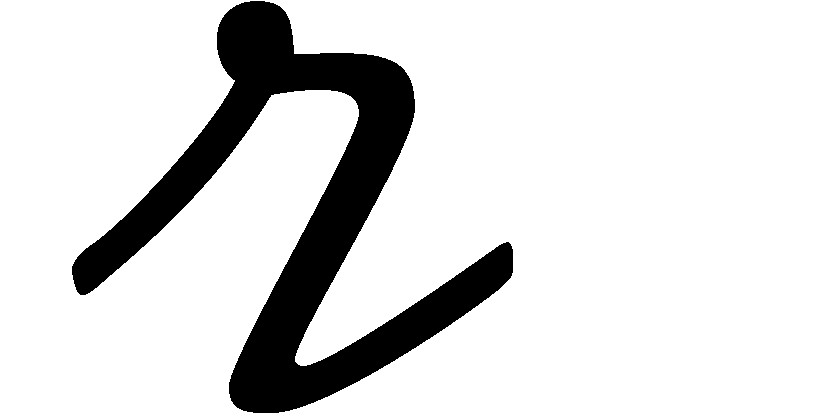
\includegraphics[trim= 1em 0 14em 0,clip]{ScriptR}}$}}}
\def\br{{\mbox{$\resizebox{.09in}{.08in}{
\includegraphics[trim= 1em 0 14em 0,clip]{BoldR}}$}}}

\newcommand{\unit}[1]{\;\;\mathrm{#1}}

\title{Electromagnetism}
\author{Richard Robinson}
\begin{document}
\maketitle
\setlength{\parindent}{0pt}

%-------------------------------------------

\chapter{Electrostatics}

\section{Electric Forces}
\textsc{In Electrodynamics}, there is typically a \emph{source point} $\b r '$ where a charge is located and a \emph{field point} $\b r$ where a field is calculated at. The \emph{seperation vector} is defined as
\begin{equation}
  \br \equiv \b r - \b r ' \qquad \hat\br = \br/\r
\end{equation}
upon definition of a coordinate system. Coulomb's law expresses the force of charges $q_i$ on another charge $q_0$, given by
\begin{equation}
    \b F \equiv K \sum \frac{q_0q_i}{\r^2} \hat\br = q_0 \b E
\end{equation}
When calculating the force via $E$, the charge density must be replaced by the respective equation. The charge differential is defined as
\begin{equation}
    dq \mapsto \lambda \, dx \sim \sigma \, dA \sim \rho \, dV
\end{equation}
When evaluating the results of the integration, the limiting cases such as $a \gg b$ can be found by evaluating the expression for $b = 0$.

\section{Electric Field}
The electric field at a point $P$ which acts like a positive test charge of a set of source charges is defined as
\begin{equation}
    \b E (\b r) \equiv K \sum \frac{q_i}{\r_i^2} \hat\br_i = K \int \frac{1}{\r ^2} \hat\br \; dq = \nabla V
\end{equation}
For most cases, symmetry can be utilized such that
\begin{equation}
    \b E = E_x \to \hat{\br} = \cos \theta
\end{equation}
An electric dipole describes the configuration of two opposite charges $q$ a distance $d$ apart. The electric dipole moment is defined as $p = qd$ towards $+q$, which means for $x \gg d$, then $E = 2Kp/ \r ^3$.

\section{Torque}
The torque of an electric dipole is defined to be
\begin{equation}
    \tau = (qE)d \sin \theta = \b p \times \b E
\end{equation}
assuming its direction is perpendicular to and into the page. The work done by the external field in turning a dipole is thus
\begin{equation}
    W = - \int_\theta \tau \; d \theta = pE(\Delta \cos \theta)
\end{equation}
which is related to the change in potential energy via
\begin{equation}
    U = - W = - \b p \cdot \b E
\end{equation}

\section{Gauss' Law}
Gauss' Law states the flux is the rate of change of an electric field of a Gaussian surface; that is,
\begin{equation}
    \Phi_E = \oint \b E \cdot d \b A = q / \epsilon_0
\end{equation}
meaning for each infinitesimal point for a given surface, $\b E$ is in the direction of the filed lines, and $\b A$ is normal to the surface. Note the "edge" of a Gaussian surface is equivalent to a single point $P$ a distance $r$ from $E$.

\bigskip
This results in $\Phi_E = 0$ if such closed surface does not enclose any charges and/or $\sum q = 0$. Because of this, $E$ for regions of infinite dimensions can be calculated via \begin{equation}
    \sum EA = q / \epsilon_0 \qquad q \mapsto \lambda x \sim \sigma A \sim \rho V
\end{equation}
For a conductor, the field $E = \sigma / \epsilon_0$.

\chapter{Electrodynamics}

\section{Potential Energy}
The difference in potential energy is defined to be \begin{equation}
    \Delta U = - \int_a^b \b F \cdot d \b s = Kq_1q_2 \left( \frac{1}{r_b} - \frac{1}{r_a} \right)
\end{equation}
Incidentally, the total potential energy of a system is \begin{equation}
    U = K \sum \sum \frac{q_iq_j}{r_{ij}}
\end{equation}
These are not to be confused with the potential difference, defined as \begin{equation}
    \Delta V = - \int_a^b \b E \cdot d \b s = \Delta U / q_o = Ed \unit{V}
\end{equation}
which is analogous to the potential energy for a point. Lastly, the electric potential is defined to be \begin{equation}
    V = K \sum \frac{q_i}{r_i} = K \int \frac{dq}{r} \sim \frac{K p \cos \theta}{r^2}
\end{equation}

\section{Electrical Properties}
The electric current $i$ is defined as the net charge flowing through a surface, \begin{equation}
    i = \frac{dq}{dt} = \int \b j \cdot d \b A
\end{equation}
where $j$ is the current density and is in the direction of $+q$ which may also be found via \begin{equation}
    \b j = - en \b v_d = \sigma \b E
\end{equation}
The resistance of a material relates the potential difference to the current through \begin{equation}
    R = \frac{\Delta V}{i} = \rho \frac{L}{A} \;\;\Omega
\end{equation}

\section{Capacitance}
The capacitance of a circuit relates the potential difference with the charge via \begin{equation}
    C = q / \Delta V \unit{F}
\end{equation}
and is only a geometrical factor. This means for a capacitive sphere, $C = 4 \pi \epsilon_0 r$. For a parallel plate capacitor, capacitance is found via  \begin{equation}
    \Delta V = \int_+^- E \; ds = \frac{\sigma d}{\epsilon_0} \iff C = \frac{\epsilon_0 A}{d}
\end{equation}
as the electric field for a plate $E = \sigma / 2 \epsilon_0$ and $\sigma = q/A$ and $C = q/\Delta V$. Likewise, the capacitance of spherical and cylindrical capacitors can be found from the result of their respective potential difference equations.

\section{Capacitors}
In a parallel circuit, the following equations hold: \begin{equation}
    q = \sum q_i = C_{eq} \Delta V \iff C_{eq} = \sum C_i
\end{equation}
and in series the converse is true: \begin{equation}
    \Delta V = \sum \Delta V_i = q / C_{eq} \iff C_{eq}^{-1} = \sum C_i^{-1}
\end{equation}
The total potential energy stored in such capacitor is defined as \begin{equation}
    U = C^{-1} \int_0^q q \; dq = \textstyle{\frac{1}{2}} C (\Delta V)^2
\end{equation}
More specifically, the energy itself is stored in the field present in such region. Similarly, the energy density is the stored energy per unit given as \begin{equation}
    u = U/Ad = 0.5 \epsilon_0 E^2
\end{equation}
For a capacitor with a dielectric of constant $\kappa$, Gauss' law gives \begin{equation}
    \epsilon_0 \oint \b E \cdot d \b A = \frac{1}{\kappa} \iff \epsilon_0 \oint \kappa \b E \cdot d \b A = q
\end{equation}

\chapter{DC Circuits}
Please see \textit{Electric Circuits} which entirely comprises this chapter itself, available with other titles at \url{http://bit.ly/eecsbooks}.

\chapter{Magnetostatics}

\section{Magnetic Field}

For particles in a magnetic field, the magnetic force is defined as \begin{equation}
    \b F_B = q \b v \times \b B = |q|vB \sin \phi
\end{equation}
However, if both an electric and magnetic field act upon a charge, the Lorentz force is \begin{equation}
    \b F = \b F_E + \b F_B = q \b E + q \b v \times \b B
\end{equation}
If both fields and the velocity vectors are tri-perpendicular in the $xyz$-plane, then the electric and magnetic force are in opposite directions, meaning \begin{equation}
    qE = qvB \iff v = E/B
\end{equation}
This configuration is known as a velocity selector, as only particles with such velocity $v$ can pass through unaffected.

\end{document}
